
\documentclass[letterpaper, 10 pt, conference]{ieeeconf}  
\IEEEoverridecommandlockouts                             
\usepackage{graphicx} 
\usepackage{hyperref}

\overrideIEEEmargins

\title{\Huge Target Tracking}
\author{Jiyu Tian} 

\begin{document}

\maketitle
\thispagestyle{empty}
\pagestyle{empty}

%-------------------------------------------------------------------------

\section{INTRODUCTION}
The Circulant Matrix (CM) tracker is very efficient finding a translated copy of the target template from the previous frame by computing many convolutions in a single shot. This is accomplished by finding the peak response of a filter applied to a region of the current frame that is expected to include the target. This filter changes from frame to frame and it is computed based on the FFT of a larger region which contains the target in the current frame. Efficiency is obtained by applying this filter in the frequency domain. 



%-------------------------------------------------------------------------
\section{ALGORITHMS DESCRIPTION}




%-------------------------------------------------------------------------
\section{EXPERIMENTAL RESULTS}




\subsection{Limitation}

%-------------------------------------------------------------------------
\section{CONCLUSION}
In this project, we implemented CM tracker. We also explored influence from various parameters, as well as the limitation of the method.
\vfill

\end{document}


\newpage

\begin{figure}[thpb]
\centering
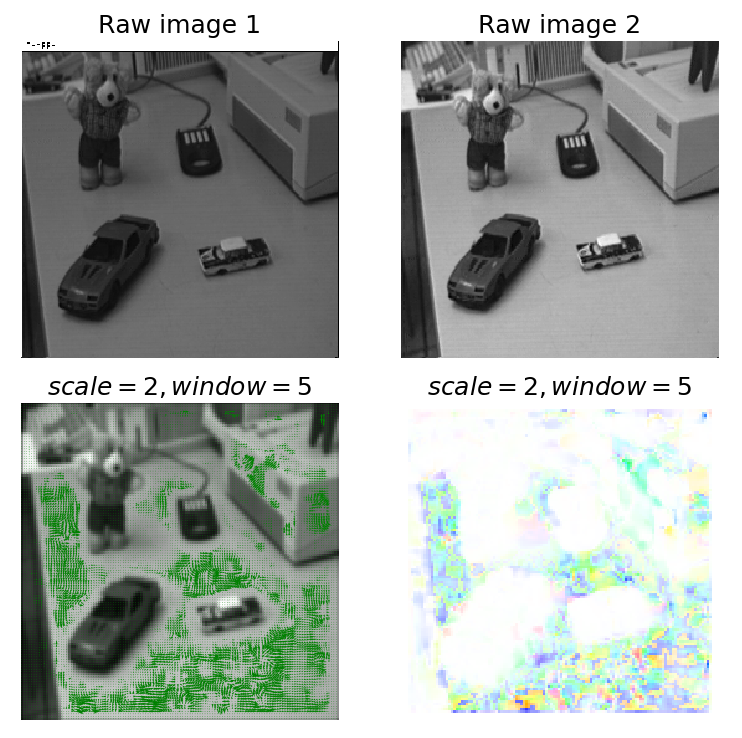
\includegraphics[width=0.415\textwidth]{limit.png}
\caption{Limitation}
\label{limit}
\end{figure}